
\section{Results}

\begin{figure*}[htbp]
	\centering
	\subfigure[espresso]{
		\label{fig_10_1}
		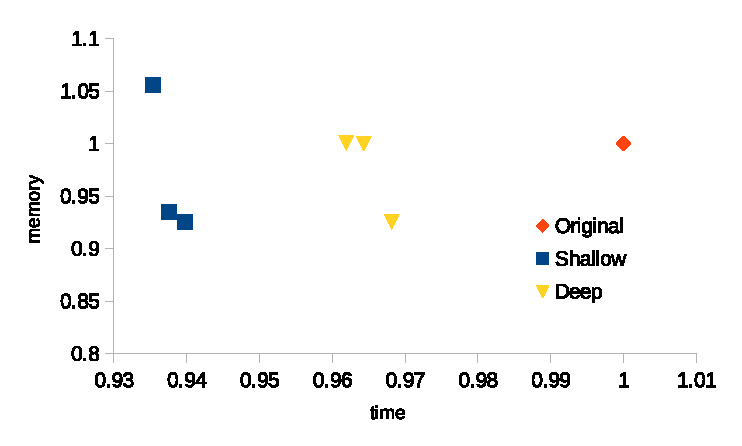
\includegraphics[width=0.4\textwidth]{fig10}
	}
	\subfigure[space]{
		\label{fig_10_2}
		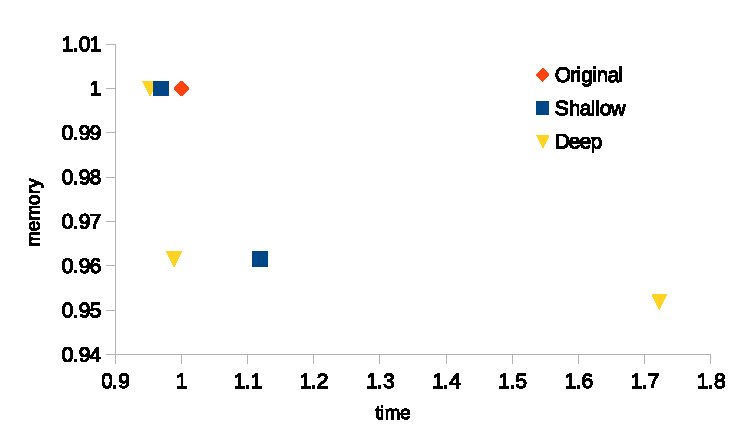
\includegraphics[width=0.4\textwidth]{fig12}
	}
	\subfigure[cfrac]{
		\label{fig_10_3}
		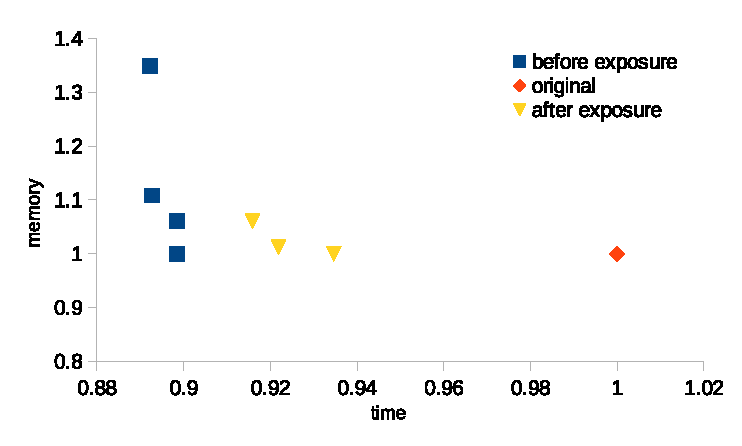
\includegraphics[width=0.4\textwidth]{fig13}
	}
	\subfigure[gawk]{
		\label{fig_10_4}
		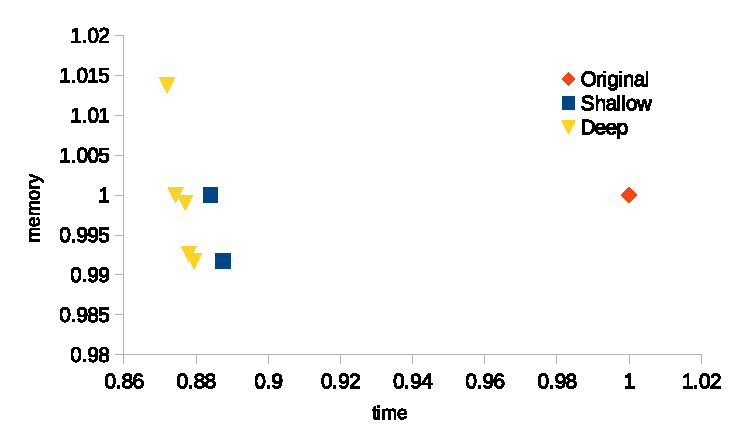
\includegraphics[width=0.4\textwidth]{fig14}
	}
	\caption{Pareto-best individuals for each application, ``before exposure'' points are abtained without tuning TOP\_FOOT\_SIZE and ``after exposure'' points with TOP\_FOOT\_SIZE tuned. Less memory and time is better.}\label{fig_10}
\end{figure*}

\subsection{Shallow Parameter Tuning Improvement}

In order to understand whether we can improve an application by specialize \emph{dlmalloc}, and whether our search-based algorithm is effective on this problem, we first conduct Shallow Parameter Tuning on \emph{dlmalloc} and compare the results with the performance of the default and randomly generated configurations. The result is reported in Table \ref{tab_2}. By Shallow Parameter Tuning, we consistantly achieve better performance in terms of time or memory on most of the applications except the memory consumption of \emph{cfrac}. This result indicates that the general-purpose allocator can be improved by adjusting it to a specific application. On the other hand, we can always find better solutions than the random search within the same computation cost. (**How much did we improve comparing to random? add data later) It proves that our multi-objective optimization of the shallow parameters is effective on this problem.

\subsection{Deep Parameter Tuning Improvement}

Knowing the Shallow Parameter Tuning works on this optimisation problem, we also want to know how much more can we achieve by the Deep Parameter Tuning. So we expose the most influential peices of code as tunable parameters and optimize them as well as the shallow parameters. From the result in Figure \ref{fig_10}, we achieve up to 11\% reduction on the time consumption (gawk, Figure \ref{fig_10_4}), and 7.5\% reduction on the memory consumption (espresso, Figure \ref{fig_10_1}), compared to the default configuration. (**How much more did we improve comparing to Shallow Parameter Tuning?) For some applications, we find that the time and memory performance can be improved at the same time. On the other hand, for some other applications, we can't find better configuration, implying the default configuration might already be the optimal for these applications. What's interesting is, by the Deep Parameter Tuning, we are able to find more extreme performance that widens the Pareto front. This means we could provide wider range of choices to users especially when the application has to run in an extreme environment. We also find that, different applications, the optimal configuration for one application don't guarantee to improve other applications, showing that the default configuration is the result of negotiation between general applications.

\begin{table*}[hbtp]
\centering
\caption{Best individuals for each application. The square points in each graph are the non-dominated best individuals of the Deep Parameter Tuning, and the triangle points are the result of the Shallow Parameter Tuning.}
\label{tab_2}
\resizebox{0.8\textwidth}{!}{
\begin{tabular}{c|c|c|c|c}
\hline
\textbf{\emph{espresso}} & time(s) & normalized time & memory(kB) & normalized memory \\
\hline
original & 4.773 & 100\% & 5152 & 100\% \\
\hline
most-time-saving before exposure & 4.667 & 97.8\% & 5440 & 105.6\% \\
\hline
most-time-saving after exposure & 4.638 & 97.2\% & 6272 & 121.7\% \\
\hline
most-memory-saving before exposure & 4.689 & 98.2\% & 4768 & 92.5\% \\
\hline
most-memory-saving after exposure & 4.654 & 97.5\% & 4768 & 92.5\% \\
\hline
\hline
\textbf{\emph{space}} & time(ms) & normalized time & memory(kB) & normalized memory \\
\hline
original & 19.3 & 100\% & 416 & 100\% \\
\hline
most-time-saving before exposure & 18.7 & 96.9\% & 416 & 100\% \\
\hline
most-time-saving after exposure & 18.0 & 93.2\% & 416 & 100\% \\
\hline
most-memory-saving before exposure & 21.6 & 111.8\% & 400 & 96.2\% \\
\hline
most-memory-saving after exposure & 39.9 & 206.3\% & 396 & 95.2\% \\
\hline
\hline
\textbf{\emph{cfrac}} & time(s) & normalized time & memory(kB) & normalized memory \\
\hline
original & 1.071 & 100\% & 332 & 100\% \\
\hline
most-time-saving before exposure & 0.956 & 89.2\% & 448 & 134.9\% \\
\hline
most-time-saving after exposure & 0.981 & 91.6\% & 352 & 106\% \\
\hline
most-memory-saving before exposure & 0.962 & 89.8\% & 332 & 100\% \\
\hline
most-memory-saving after exposure & 1.001 & 93.5\% & 332 & 100\% \\
\hline
\hline
\textbf{\emph{gawk}} & time(s) & normalized time & memory(kB) & normalized memory \\
\hline
original & 2.711 & 100\% & 4356 & 100\% \\
\hline
most-time-saving before exposure & 2.396 & 88.4\% & 4356 & 100\% \\
\hline
most-time-saving after exposure & 2.389 & 88.1\% & 4320 & 99.2\% \\
\hline
most-memory-saving before exposure & 2.406 & 88.8\% & 4320 & 99.2\% \\
\hline
most-memory-saving after exposure & 2.389 & 88.1\% & 4320 & 99.2\% \\
\hline
\end{tabular}}
\end{table*}

\subsection{Understanding the Exposed Parameters}

\begin{table*}[htbp]
\centering
\caption{Exposed Parameters}
\label{tab_exposed_param}
\resizebox{\textwidth}{!}{
\begin{tabular}{|c|c|c|c|}
\hline
Line & Exposed part & Substitute options & Description \\
\hline
4059 & (use\_mmap(m) \&\& nb >= mparams.mmap\_threshold \&\& m->topsize != 0) & 2 & Enable \emph{mmap} system call\\
\hline
4144 & (m->footprint\_limit == 0 || (fp > m->footprint \&\& fp <= m->footprint\_limit)) & 4 & Predicate controling system allocation\\
\hline
4348 & TOP\_FOOT\_SIZE & numeric & Segment overhead size of the top chunk\\
\hline
4353 & ((m->topsize - pad + (unit - SIZE\_T\_ONE)) / unit - SIZE\_T\_ONE) * unit & 6 & Calculation of remaining memory when trimming\\
\hline
\end{tabular}}
\end{table*}
From the sensitivity information, we find four places that have the most impact to the performance of \emph{dlmalloc}, which are list in Table \ref{tab_exposed_param}. They locate in different functions that involve system allocation and deallocation. LINE4059 checks whether current situation meets the \emph{mmap} criteria, so it could easily enable or disable direct memory mapping. LINE4144 is also a predicate controling the extending of the heap. TOP\_FOOT\_SIZE in LINE4383 is a constant determined by some other macros and parameters. It influences how much memory should be always kept in the top chunk. LINE4353 is an expression calculating how much memory should be preserved when shrinking the heap.

After human inspection, one can easily find the exposed parameters introduced above can directly influence the memory and/or time performance of the allocator. Due to the limit space, we only elaborate one of them. TOP\_FOOT\_SIZE controls how many extra bytes should be included in the top chunk while the allocator extends the top chunk. It influences how much more memory than actually needed \emph{dlmalloc} should keep to buffer allocation and deallocation. Bigger TOP\_FOOT\_SIZE tends to cost more memory but possibly saves some costly system allocation and deallocation. The optimal value could vary across applications. Originally it is a constant determined by some macros and system related parameters. After made to a tunable parameter and exposed to users, it can be explicitly configured from the outside like other parameters.
